% GO TO: /Users/leonlufkin/Library/texmf/tex/latex
%        to add custom packages to the path
\documentclass{article}
\usepackage{report}

\title{Interpreting Dynamics}
\author{Leon Lufkin}
\date{\today}

\makeatletter
\let\Title\@title
\let\Author\@author
\let\Date\@date

\begin{document}

%%%%%%%%%%%%%
%% Setting %%
%%%%%%%%%%%%%
\section{Setting}
We can mostly explain symmetry breaking and tiling, and so we finally want to explain localization.
To do this, I focus on a single-neuron model with ReLU activation.

The task is to discriminate between two classes of inputs:
\begin{align}
  X_1 \sim p(\xi_1), \quad X_0 \sim p(\xi_0),
\end{align}
which are $n$-dimensional vectors.
We only assume that $p$ is \emph{translation-invariant} (this is explained more below).
Every input $X_i$ has scalar label $Y_i$.
The distribution $p$ is paramaterized by $\xi > 0$, which defines the length-scale of correlations in the input.
Specifically, we construct $p$ so that
\begin{align}
  \operatorname{Cov}(X) = \Sigma(\xi), \quad \Sigma(\xi)_{ij} = \exp(-(i-j)^2 / \xi^2).
\end{align}

% \begin{figure}[!ht]
%   \centering
%   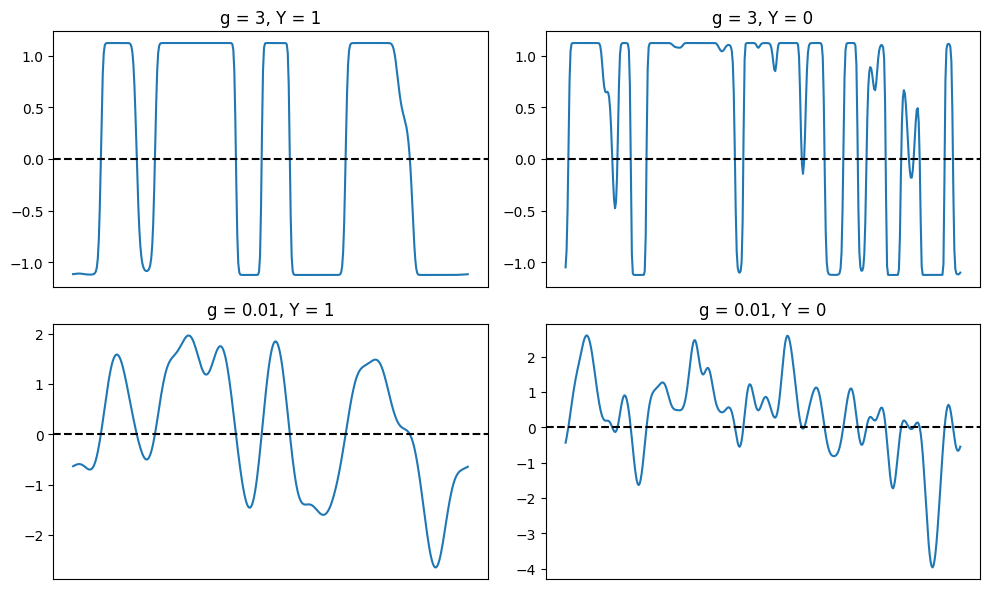
\includegraphics[width=0.7\textwidth]{figs/samples.png}
% \end{figure}

% We train a two-layer neural network on this task using gradient descent.
% \begin{align}
%   \hat{y}(x) = \frac{1}{K} \sum_{k=1}^{K} \sigma(\langle w_k, x \rangle + b_k),
% \end{align}
% \begin{figure}[!ht]
%   \centering
%   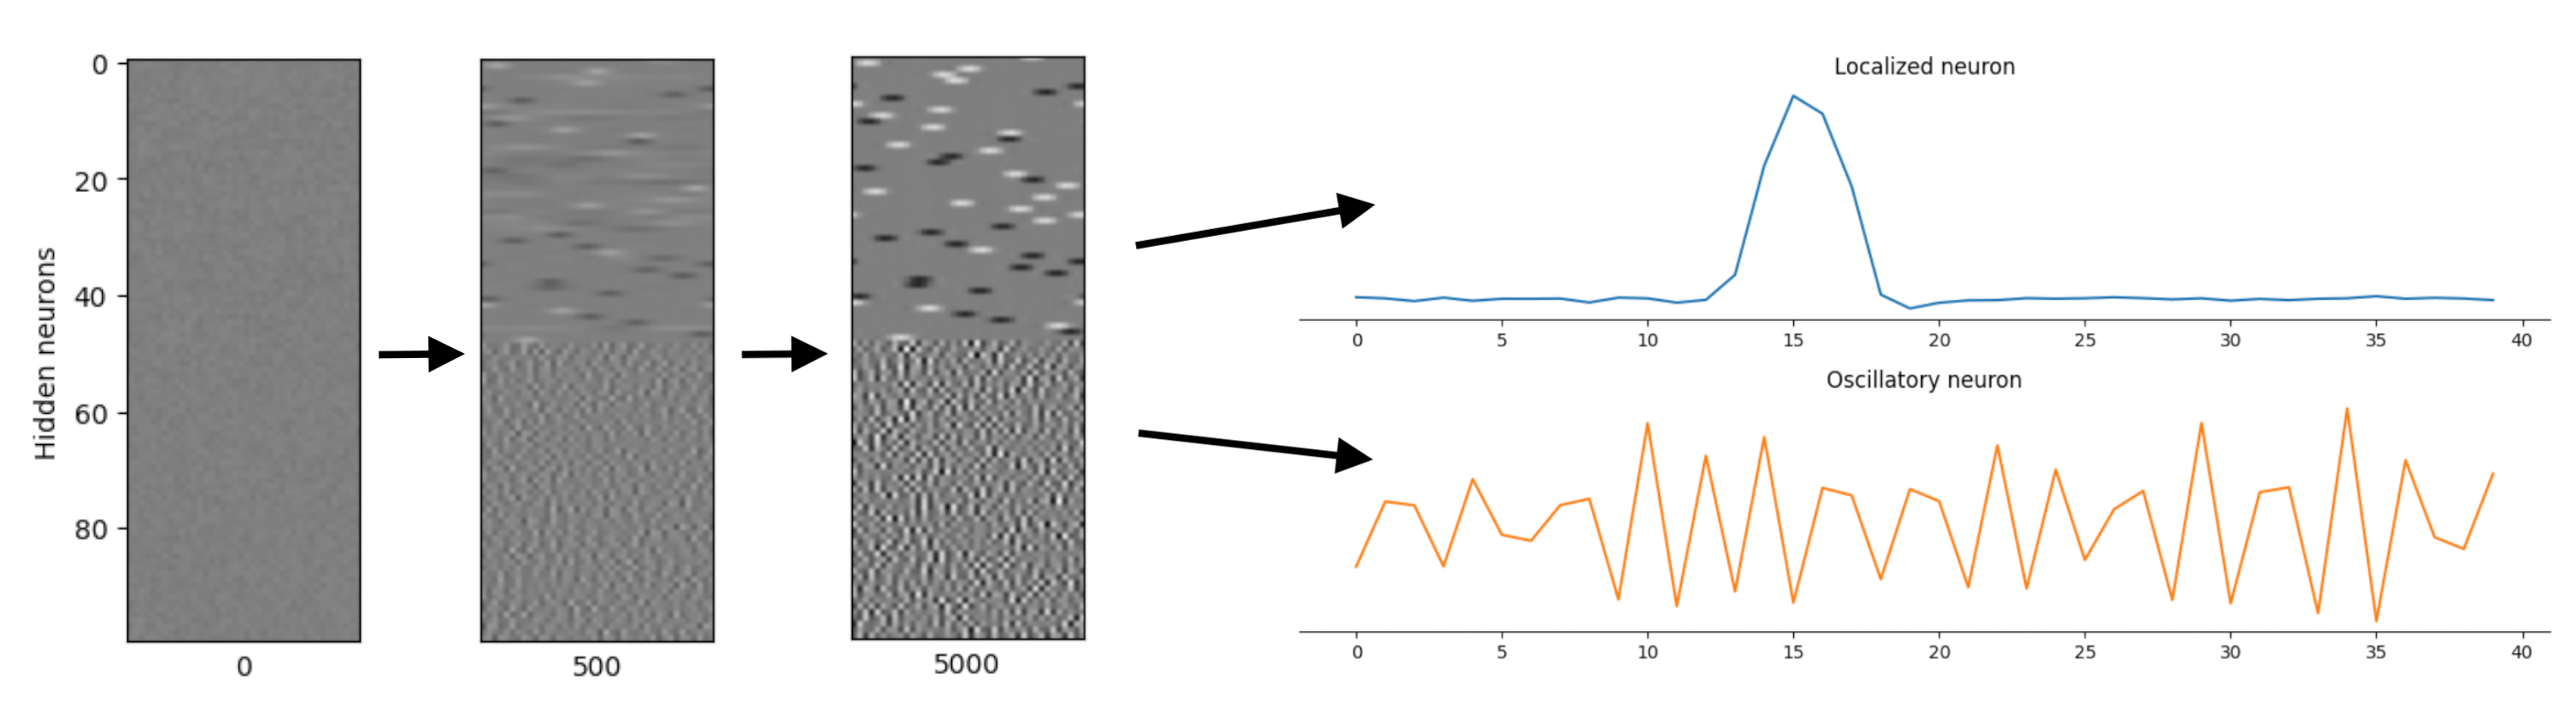
\includegraphics[width=\textwidth]{figs/fig_rfs_arrows.png}
% \end{figure}

We consider one neuron without bias and ReLU activation.
\begin{align}
  \hat{y}(x) = \operatorname{ReLU}(\langle w, x \rangle),
\end{align}
where $w$ is our receptive field.

%%%%%%%%%%%%%%
%% Dynamics %%
%%%%%%%%%%%%%%
\section{Dynamics}
The dynamics of $w$ is given by
\begin{align}
  \tau \frac{d}{dt} w
  &= - \frac{\partial \LL}{\partial w}
  = \frac{1}{2} \underbrace{ \left[ \frac{\partial}{\partial w} \E_{ X \mid Y = Y_i } \left[ \operatorname{ReLU}(\langle w, x \rangle) \right] \right] }_{\triangleq f(w)} - \frac{1}{2} ( \Sigma_0 + \Sigma_1 ) w,
\end{align}
where $i$ is the class with output label 1, i.e. $Y_i = 1$ and $Y_{1-i} = 0$.
This elucidates some universal structure.
We could also write $f$ as
\begin{align}
  f(w) &= \E_{ X \mid Y = Y_i } \left[ \mathbbm{1}(\langle w, X \rangle \geq 0) X \right]. \label{eq:f}
\end{align}
This lets us establish some properties of $f$.
\begin{enumerate}
  \item \emph{It is invariant to scaling $w$}: $f(w) = f(\alpha w)$ for $\alpha > 0$.
  \item \emph{It is sign equivariant}: $f(-w) = -f(w)$.
  \item \emph{It is translation equivariant\footnote{Here, ``translation'' refers to shifts of the \emph{entries} of a vector. So, if $\CC$ is a shift down by 1, $x_i = (\CC x)_{i+1}$}}: $f(\CC w) = \CC f(w)$, where $\CC$ is a circular shift.
  \item \emph{It can preserve symmetry in $p$}: If $p$ is symmetric w.r.t. some invertible linear  transformation $A$, i.e. $p_{\xi}(x) = p_{\xi}(A x)$ for all $x$, then $f(A w) = A^{-\top} f(w)$~\footnote{If $A$ is orthogonal, then $f(A w) = A f(w)$.}.
\end{enumerate}
(Note property 4 captures properties 2 and 3.)
Thus, \underline{$f$ only depends on the shape of $w$, not it's magnitude or position}.
So, it is precisely the object we need to understand.

The above equation also makes precise why a Gaussian approximation empirically always holds early in training.
Early on, with $w$ initialized as standard Gaussian, the second term dominates the dynamics.
Note this term looks a lot like the update rule if we assume $p$ is Gaussian.
This term shrinks the receptive field, specifically shrinking lower-frequency oscillations faster than higher-frequency ones\footnote{Does this make sense?}.
Once $w$ becomes sufficiently small in norm so that the second term is on the order of $f(w)$, the first term is no longer negligible, and the dynamics are no longer Gaussian.

For certain distributions, we can evaluate $f(w)$ exactly, or at least find its form and interpret it.
For Gaussian data,
\begin{align*}
  f(w) &= \frac{1}{\sqrt{2\pi}} (w^\top \Sigma_i w)^{-\frac{1}{2}} \Sigma_i w.
\end{align*}
For elliptical data more generally,
\begin{align*}
  f(w) &= g(w^\top \Sigma_i w) \Sigma_i w,
\end{align*}
where $g : \R_{\geq 0} \to \R_{\geq 0}$ is some scalar function that scales like $\sim x^{-\frac{1}{2}}$ for inputs $x$.
Given this form, we can write the update in Fourier space, given by $u = P^\top w$, where $P$ is the (real) DFT matrix.
\begin{align}
  \tau \frac{d}{dt} u
  &= g(u^\top \Lambda_i u) \Lambda_i u - \frac{1}{2} ( \Lambda_0 + \Lambda_1 ) u,
\end{align}
where the $\Lambda_i$ are diagonal matrices of eigenvalues of $\Sigma_i$.
Because this is diagonal, we can compute steady states, which lets us show that the limiting solutions are a superposition of just one or two modes (i.e. $u$ is sparse)\footnote{I need to confirm this with simulations.}.
This is insufficient for localization, which requires $u$ to be sparse in the \emph{spatial} domain, not the Fourier domain.

In general, it's hard to say much more about $f$.
I don't know what it looks like for Alessandro's data model.
\textbf{I want to empirically investigate how it behaves.}
I think we can do this using Jax, but I'm not sure what the right questions to ask are or how to answer them.


\paragraph*{Extra fact}
One additional thing we can say about $f$ is that
\begin{align*}
  \frac{\partial}{\partial w} f(w)_i \perp w \quad \forall i,
  \qquad \text{and} \qquad
  \frac{\partial}{\partial w_j} f(w) \perp w \quad \forall j.
\end{align*}
This is either something important about interpreting $f$ or entirely obvious.
Not sure which, but this seems like a special consequence of using ReLU activation.
To see why:
\begin{align*}
  \frac{\partial}{\partial w_j} f(w)_i
  &= \frac{\partial}{\partial w_j} \frac{\partial}{\partial w_i} \int_{\R^n} p_{\xi}(x) \operatorname{ReLU}(\langle w, x \rangle) dx \\
  &= \frac{\partial}{\partial w_j} \int_{\R^n} p_{\xi}(x) \mathbbm{1}(\langle w, x \rangle \geq 0) x_i dx \\
  &= \int_{\R^n} p_{\xi}(x) \delta(\langle w, x \rangle) x_i x_j dx,
\end{align*}
where $\delta$ is the Dirac delta function.

%%%%%%%%%%%%%%%%%%%%%%%%%%
%% Signals on hypercube %%
%%%%%%%%%%%%%%%%%%%%%%%%%%
\section{Signals on the hypercube}
We will try to come up with some general sufficient conditions for localization.
Let us introduce the data model of Alessandro as a starting point.
There,
\begin{align}
  p_{\xi}(x) = \operatorname{Law}(X), \quad X_i = \frac{1}{\sqrt{\mathcal{Z}(g)}} \operatorname{erf}(g Z_i), \quad X \sim \NN(0, \Sigma(\xi)),
\end{align}
where $g > 0$ is our gain parameter and $\mathcal{Z}(g)$ is a normalization constant that ensures $\operatorname{Var}(X_i) = 1$ for all $i$.
(Note that $\operatorname{Cov}(X) \neq \Sigma(\xi)$, but it's pretty close.)
Importantly, as $g \to 0$, $X \overset{d}{\to} Z$, i.e. the data is approximately Gaussian.
However, as $g \to \infty$, $X$ becomes supported on the vertices of the hypercube $\{ \pm 1 \}^n$.
After staring at \cref{eq:f} for a while, I think that this is the key to understanding localization.
I'll explain this below, but first, some analytical examples.

\paragraph*{Single bump}
If $w = e_i$, then
\begin{align}
  f(w) = \Sigma e_i.
\end{align}

\paragraph*{Balanced bumps}
If $w = e_i + e_j$, then
\begin{align}
  f(w) = \Sigma (e_i + e_j).
\end{align}

\paragraph*{Imbalanced bumps}
If $w = \alpha e_i + e_j$ for $\alpha > 1$, then
\begin{align}
  f(w) = \Sigma e_i.
\end{align}
Interesting!

If we flip the sign of the smaller bump so that
If $w = \alpha e_i - e_j$ for $\alpha > 1$, then
\begin{align}
  f(w) = \Sigma e_i.
\end{align}
Cool!

\paragraph*{Three bumps}
If $w = \alpha e_i + \beta e_j + e_k$ for $\alpha > \beta > 1$, then
\begin{align}
  f(w) \approx \Sigma e_i.
\end{align}

\paragraph*{More generally?}
Assume $w_1 > 0$.
\begin{align*}
  \mathbbm{1}(\langle w, x \rangle \geq 0)
  &= \mathbbm{1}( x_1 \geq - \sum_{i=2}^{n} ( \tfrac{w_i}{w_1} ) x_i ).
\end{align*}
If $\sum_{i=2}^{n} | \tfrac{w_i}{w_1} | < 1$, this is equivalent to $\mathbbm{1}(x_1 \geq 0) = \mathbbm{1}(x_1 \geq 1)$.
This is a pretty strong condition on $w$ that is not usually true.
However, it gives us a starting point for how we might be able to generally cut away a lot of the complexity of $f$ when the data is supported on the vertices of the hypercube.

Let's consider some separation point $k$, (recall we assume $|w_1| > \ldots > |w_n|$, but this is just to make the sums easier to write—we just need to partition the entries of $w$ into two sets).
\begin{align*}
  \mathbbm{1}(\langle w, x \rangle \geq 0)
  &= \mathbbm{1}( \sum_{i=1}^{k} w_i x_i \geq - \sum_{i=k+1}^{n} w_i x_i ).
\end{align*}
What is the smallest positive value the LHS produces?
Define
\begin{align}
  \delta &\triangleq \min_{x \in \{ \pm 1 \}^k} \left| \sum_{i=1}^{k} w_i x_i \right|. \label{eq:delta}
\end{align}
Then, if $\left| \sum_{i=k+1}^{n} w_i x_i \right| < \delta$ for all $x$, which in this case is equivalent to $\sum_{i=k+1}^{n} \left| w_i \right| < \delta$, we have
\begin{align*}
  \mathbbm{1}(\langle w, x \rangle \geq 0)
  &= \mathbbm{1}( \sum_{i=1}^{k} w_i x_i \geq 0 ).
\end{align*}

We want $\X$ s.t. we can make $k$ small in the following inequality.
\begin{align*}
  \min_{x \in \X} \left| \sum_{i=1}^{k} w_i x_i \right| > \max_{x \in \X} \left| \sum_{i=k+1}^{n} w_i x_i \right| 
\end{align*}


Again, we're making \emph{universal statements} about $f$ without assuming the underlying probability distribution (other than that it's supported on the hypercube).
In practice, we can do better than having $x$ in \cref{eq:delta} range across the entire $k$-dimensional hypercube, \emph{considering instead some subset of it that occurs with high probability under $p$}.
This would allow us to cut away even more of the complexity of $f$.
Obviously, we'd want to consider the smallest $k$ such that the condition above holds.

If $k$ is sufficiently small, then we can cut away a lot of the complexity of $f$.
More specifically, if $w_i$ is sufficiently small, the indicator function treats it as if it were zero.
However, we need to understand how the remaining terms, which cannot be treated like zero, affect the indicator function.

\subsection*{SDP}
\Cref{eq:delta} is related to the integer optimization problem
\begin{align*}
  \delta_\text{INT} &\triangleq \max_{x \in \{ \pm 1 \}^k} \sum_{i,j=1}^{k} A_{ij} x_i x_j,
\end{align*}
where $A = -w w^\top$.
This is because $\sum_{i,j=1}^{k} A_{ij} x_i x_j = (x^\top A x) = - (\langle w, x \rangle)^2$.
So,
\begin{align*}
  \delta_\text{INT}
  &= \max_{x \in \{ \pm 1 \}^k} - (\langle w, x \rangle)^2
  = - \min_{x \in \{ \pm 1 \}^k} (\langle w, x \rangle)^2
  = - \sqrt{\delta}.
\end{align*}
It would be cool to bound $\delta$ from below in terms of $w$.
Grothendieck's inequality might let us do this, albeit with a rather loose bound.


\subsection{Simulations}
In the few examples above, we've been able to show analytically that, because $X$ has support on the hypercube, $f$ extracts the maximum value of $w$.
This makes a lot of sense!
But we'd like to show this in a more general setting.

Something like $X_j$ is approximately independent of $\mathbbm{1}( \langle w, X \rangle \geq 0 )$ when $j$ does not correspond to the maximum absolute entry in $w$.
Otherwise, $X_j \approx \sgn(w_j)$.

Let's consider the set of $x$



\begin{align}
  \E_X[ \mathbbm{1}(\langle w, x \rangle \geq 0) X ]
  &= \E_X\left[ \sum_{ x' \in \Theta } \mathbbm{1}(X = x') X\right] \\
  &= \E_X\left[ \sum_{ x' \in \Theta } \left[\prod_{i=1}^{n} \mathbbm{1}(X_i = x_i')\right] X\right] \\
  &= \E_X\left[ \sum_{ x' \in \Theta } \left[\prod_{i=1}^{n} \frac{\sgn(x_i')}{2}( X_i + x_i' ) \right] X\right] \\
  &= \sum_{ x' \in \Theta } \E_X\left[ \left(\prod_{i=1}^{n} \frac{\sgn(x_i')}{2}( X_i + x_i' )\right) X\right].
\end{align}
Entrywise,
\begin{align*}
  \sum_{ x' \in \Theta } \E_X\left[ \left(\prod_{i=1}^{n} \frac{\sgn(x_i')}{2}( X_i + x_i' )\right) X_j \right]
  &= \sum_{ x' \in \Theta } \E_X\left[ \left(\prod_{i=1}^{n} \frac{\sgn(x_i')}{2}( X_i + x_i' ) X_j \right) \right] \\
\end{align*}

First, I want to understand how we could rigorously apply this intuition to simplify $f$.
Let's start by defining the event
\begin{align}
  \Theta
  &= \big\{ x = (x_j)_{j\in[n]} \in \{ \pm 1 \}^n \mid \langle w, x \rangle \geq 0 \big\}.
\end{align}
Then,
\begin{align}
  \mathbbm{1}(\langle w, x \rangle \geq 0)
  &= \sum_{ x' \in \Theta } \mathbbm{1}(x = x')
  = \sum_{ x' \in \Theta } \prod_{j \in [n]} \mathbbm{1}(x_j = x_j')
  % = \sum_{j \in [n]} \sum_{ x' \in \Theta } \mathbbm{1}(x_j = x_j').
\end{align}
So,
\begin{align}
  \E_{X \mid Y=1}\left[ \mathbbm{1}(\langle w, X \rangle \geq 0) X \right]
  % &= \E_{X \mid Y=1}\bigg[ \bigg( \sum_{j \in [n]} \sum_{ x' \in \Theta } \mathbbm{1}(X_j = x_j') \bigg) X \bigg] \\
  &= \sum_{j \in [n]} \E_{X \mid Y=1}\bigg[ \bigg( \underbrace{ \sum_{ x' \in \Theta } \mathbbm{1}(X_j = x_j') }_{\triangleq g_j(X)} \bigg) X \bigg].
\end{align}
% We want to show $g_j(x) \approx 1$ for $j > 1$ (or, more generally, $j$ for which $w_j$ is not sufficiently large).
% More specifically,
With this perspective, we want to show
\begin{enumerate}
  \item $g_j(x) \approx \mathbbm{1}(x_j = \operatorname{sign}(w_j))$ when $w_j$ is sufficiently large, and
  \item $g_j(x) \approx 1$ when $w_j$ is not sufficiently large.
\end{enumerate}
We also want to understand what it means for $w_j$ to be sufficiently large.
Hopefully, we can show there is a pretty clear divide between the two cases, and that nothing falls in between.
\textbf{Now, how do I do this?}

We'll start with the case where $w_j > 0$ for the sufficiently large case.

Let's consider the case where only one $w_j$ is sufficiently large.
WLOG, let's say this happens for $j = 1$.
As we make it larger, how do the $g_j(x)$ change?

Note that
\begin{align}
  g_j(x)
  &= \sum_{ x' \in \Theta } \mathbbm{1}(x_j = x_j') \\
  &= | \{ x' \in \Theta \mid x_j' = 1 \} | \mathbbm{1}(x_j = 1) + | \{ x' \in \Theta \mid x_j' = -1 \} | \mathbbm{1}(x_j = -1)
\end{align}

\end{document}
